\documentclass[conference]{IEEEtran}
\IEEEoverridecommandlockouts
% The preceding line is only needed to identify funding in the first footnote. If that is unneeded, please comment it out.
\usepackage{cite}
\usepackage{CJKutf8}
\usepackage{amsmath,amssymb,amsfonts}
\usepackage{algorithmic}
\usepackage{graphicx}
\usepackage{textcomp}
\usepackage{xcolor}
\usepackage{verbatim}
\usepackage{multicol}  
\usepackage{multirow}  
\usepackage{stfloats}
\usepackage{url}
\makeatletter
\newcommand{\rmnum}[1]{\romannumeral #1}
\newcommand{\Rmnum}[1]{\expandafter\@slowromancap\romannumeral #1@}
\makeatother
\def\BibTeX{{\rm B\kern-.05em{\sc i\kern-.025em b}\kern-.08em
		T\kern-.1667em\lower.7ex\hbox{E}\kern-.125emX}}
\begin{document}
	\begin{CJK}{UTF8}{gbsn}
	
	\title{Unsupervised Keyword Extraction Method based on Chinese Patent Clustering\\
		%\thanks{Identify applicable funding agency here. If none, delete this.}
	}

	\author{\IEEEauthorblockN{1\textsuperscript{st} Given Name Surname}
		\IEEEauthorblockA{\textit{dept. name of organization (of Aff.)} \\
			\textit{name of organization (of Aff.)}\\
			City, Country \\
			email address}
		\and
		\IEEEauthorblockN{2\textsuperscript{nd} Given Name Surname}
		\IEEEauthorblockA{\textit{dept. name of organization (of Aff.)} \\
			\textit{name of organization (of Aff.)}\\
			City, Country \\
			email address}
		\and
		\IEEEauthorblockN{3\textsuperscript{rd} Given Name Surname}
		\IEEEauthorblockA{\textit{dept. name of organization (of Aff.)} \\
			\textit{name of organization (of Aff.)}\\
			City, Country \\
			email address}
		\and
		\IEEEauthorblockN{4\textsuperscript{th} Given Name Surname}
		\IEEEauthorblockA{\textit{dept. name of organization (of Aff.)} \\
			\textit{name of organization (of Aff.)}\\
			City, Country \\
			email address}
		\and
		\IEEEauthorblockN{5\textsuperscript{th} Given Name Surname}
		\IEEEauthorblockA{\textit{dept. name of organization (of Aff.)} \\
			\textit{name of organization (of Aff.)}\\
			City, Country \\
			email address}
		\and
		\IEEEauthorblockN{6\textsuperscript{th} Given Name Surname}
		\IEEEauthorblockA{\textit{dept. name of organization (of Aff.)} \\
			\textit{name of organization (of Aff.)}\\
			City, Country \\
			email address}
	}

	\maketitle
	
	\begin{abstract}
		Recently, patent data analysis has attracted a lot of attention, and patent keyword extraction is a hot problem. Most existing methods for patent keyword extraction are based on the frequency of words without semantic information. In this paper, we propose an Unsupervised Keyword Extraction Method (UKEM) based on Chinese patent clustering. More specifically, we use a Skip-gram model to train word embeddings based on a Chinese patent corpus. Then each patent is represented as a vector called patent vector. These patent vectors are clustered to obtain several cluster centroids. Next, the distance between each word vector in patent abstract and cluster centroid is computed to indicate the semantic importance of this word. The experimental results on several Chinese patent datasets show that the performance of our proposed method is better than several competitive methods.
	\end{abstract}
	
	\begin{IEEEkeywords}
		patent keyword extraction, semantic information, patent clustering, patent vector
	\end{IEEEkeywords}
	
	\section{Introduction}
	In 2018, the number of Chinese invention patent applications was grown up to 1.542 million, and the growth rate reached 11.6\% according to the statistics of China National Intellectual Property Administration. Many patents have high economic value and are worth being protected in some important fields \cite{b1}. Inappropriate analysis of patent technology may lead to patent litigation \cite{b2}. Due to the valuable contemporary technological information that patents contained, we can discover the direction of new technologies and predict future trends in related fields by analyzing patent documents \cite{b3}. Recently, more and more text mining methods have been utilized to analyze patent documents.
	
	One important research issue in patent analysis is patent keyword extraction. Keywords can be used to summarize the corresponding text and classify documents into categories \cite{b4}. However, all Chinese patent documents have no applicant-assigned keywords, which makes artificially assigning keywords for each patent document very difficult. Therefore, we focus on the patent keyword extraction.
	
	Traditional keyword extraction algorithms can be roughly classified into supervised and unsupervised methods. In this paper, we focus on the latter.
	
	In unsupervised keyword extraction methods, most algorithms consider word frequency as a decisive factor in selecting keywords. For example, Term Frequency-Inverse Document Frequency (TF-IDF) was proposed in keyword extraction \cite{b5}. However, TF-IDF does not consider the semantic relation between words. TextRank is the typical graph-based method \cite{b6}, which is similar to the PageRank algorithm. However, due to the high computational complexity, TextRank requires much time to calculate the PageRank values of each word. Rapid Automatic Keyword Extraction (RAKE) \cite{b7} can extract key-phrases from texts rapidly, but it cannot extract semantically significant words and the accuracy is not high. Hu et al. \cite{b8} proposed the Patent Keyword Extraction Algorithm (PKEA) based on the distributed representation, it can extract semantic keywords from patent documents. However, PKEA needs a large number of pre-defined category words to determine the centroid of each patent category.
	
	In a word, most existing methods for patent keyword extraction are based on the frequency of words without semantic information. In addition, many patent clustering algorithms are based on patent citation networks \cite{b9}. In this paper, we propose an Unsupervised Keyword Extraction Method (UKEM) based on Chinese patent clustering. We consider technical field as the important section for patent clustering. More specifically, firstly, we use Skip-gram model \cite{b10} to train word embeddings based on a Chinese patent corpus, and the introduced Skip-gram model can represent the semantic and syntactic relation between words well. Secondly, we calculate the arithmetic mean of the word vectors of each patent technical field, and each vector is used to represent each patent, which called patent vector. Then we use a classical clustering algorithm to cluster related patents automatically by patent vectors, and the centroid of each cluster can be calculated easily. Finally, we predict the relevant cluster for each test patent abstract, and then the distance between each candidate word vector and the relevant cluster centroid is designed to indicate the importance of candidate words individually. The experimental results demonstrate the effectiveness of our method.
	
	Our main contributions in this paper can be summarized as follows:
	\begin{itemize}
	\item We propose an unsupervised keyword extraction method based on Chinese patent clustering, which contains semantic information. In our method, we consider technical field as the important section for patent clustering.
	\item We release a manually tagged patent keyword dataset, consisting of 600 Chinese patent documents with high-quality manually tagged keywords in several fields. This dataset is accessible in our github repository$\footnote{\url{https://github.com/NoteXYX/Manually-tagged-patent-keyword-dataset}}$.
	\end{itemize}

	The rest of the paper is organized as follows. Section \Rmnum{2} discusses related works in keyword extraction research. Section \Rmnum{3} provides a detailed description of our proposed algorithm. Section \Rmnum{4} shows our experimental results. Section \Rmnum{5} summarizes this paper and discusses future work.
	
	
	\section{Related Work}
	Keyword extraction has been playing an important role in classic text mining tasks for many years, which is the basis for text retrieval and text classification. In the field of patents, keyword extraction has received a lot of attention as an important way to obtain advanced technology from patent documents \cite{b11}. Kim, et al. \cite{b12} built a semantic network of keywords from patent documents in order to predict emerging technologies. Lee, et al. \cite{b13} found that new technological opportunities can be identified by building a patent keyword evolution map. However, all patent documents have no applicant-annotated keywords. Thus, many researchers have focused on patent keyword extraction.
	
	The first step in extracting keywords from patents is to decide the most appropriate section of the patent documentation for keyword extraction. Patent documents are divided into multiple sections, including title, abstract, claims, and description. The number of words in these sections is quite different from each other because of their different purposes. Noh, et al. \cite{b14} proposed guidelines for extracting keywords. They evaluated the keyword extraction performance considering different sections of patents. They found that the most suitable keyword extraction strategy for patent research is selecting words from the abstract section.
	
	The second phase is to determine the keyword extraction algorithm. Generally, based on whether a labeled corpus is required, existing keyword extraction algorithms can be roughly classified into supervised and unsupervised methods.
	
	In supervised keyword extraction methods, a large number of tagged keywords are required for training a classifier. This classifier determines which words in the document are important. Many commonly used classification algorithms have been tried. Ardiansyah et al. \cite{b15} extracted valuable information from trained neural networks by using decision tree. Domoto et al. \cite{b16} proposed a spoken term detection method using SVM-based classifier. This SVM-based classifier was trained with a large number of pre-indexed keywords. Yu et al. \cite{b17} proposed a new Hidden-State Maximum Entropy (HSME) model for estimating word confidence. Their method outperforms decision tree and SVM in most keyword-spotting tasks. Liu et al. \cite{b18} proposed a semi-automatic method based on partitioning corpus to extract technology effect phrases in Chinese patent abstracts. Their method needs a few manually extracted patent abstracts to construct a domain-independent corpus.
	
	Unsupervised keyword extraction methods can be divided into statistical methods, neural network based methods, and graph-based methods. Nam et al. \cite{b19} proposed a keyword based method that can monitor the adoption of existing technology by term frequency-inverse document frequency (TF-IDF) and K-means clustering using cited patents. When the number of patents using TF-IDF and K-means clustering was too small, they considered patents that were cited by the originally set of patents. This method is suitable for US patents but not for Chinese patents because Chinese patents have no cited patents. Wu et al. \cite{b20} proposed an unsupervised neural network based keyword extraction algorithm, which was inspired by the visual attention mechanism. Their algorithm can effectively extract keywords with rich contextual information from the document. Wang et al. \cite{b21} proposed a sentence-ranking model based on a sentence embedding graph and heuristic rules. Their experimental results show that keywords are likely to exist in key sentences. They believe that the importance of a sentence is related to the position of the sentence, and the importance of a word is related to the part of speech and the function of the word. Wen et al. \cite{b22} proposed a keywords graph model based on the basic idea of TextRank. They used Word2Vec to calculate the similarity between words as transition probability of nodes' weight. Li et al. \cite{b23} proposed a graph-based ranking algorithm by exploiting Wikipedia as an external knowledge base for short text keywords extraction. They pointed out that the Wikipedia's concept can be used to enrich the semantic information of each word in TextRank algorithm.
	
	In summary, the research of keyword extraction has made great progress. We are aware that patent keyword extraction has great influence on patent analysis and becomes a hot problem. However, there are only a little previous studies about keyword extraction algorithm for Chinese patents \cite{b21}. Therefore, we introduce a novel keyword extraction method for Chinese patents, and obtain the better performance than several competitive methods.
	\section{Methodology}
	\subsection{Overview of the Framework}
	The framework of our proposed UKEM is shown in Fig.~\ref{framework}, which contains a preprocessing module, a clustering module and a keyword extraction module. 
	\begin{figure}[ht]
		\centering
		\includegraphics[scale=0.6]{framework.jpg} 
		\caption{The framework of our proposed UKEM.}
		\label{framework}
	\end{figure}
	These modules will be introduced in detail next.
	
	\subsection{Preprocessing Module}
	We use a Chinese patent corpus to construct a Chinese patent database. Chinese patent documents have strict and standardized templates and writing criterions. Most previous studies have extracted keywords from patent abstracts or patent titles. In this paper, we consider abstract and technical field as two important sections in patent keyword extraction.
	
	Firstly, we extract abstract from each patent document in our Chinese patent database. We use jieba$\footnote{\url{https://github.com/fxsjy/jieba}}$ as the Chinese word segmentation tool. However, after the procedure of word segmentation, a large number of meaningless words and punctuations may be produced. Therefore, we create a stop words table to filter those meaningless words (such as “和” (and)) and punctuations (such as “.”) in extracted abstracts.
	
	Secondly, because the patent abstract has hundreds of words and clearly states the technical problems to be solved and the primary technical method adopted by the patent, the words in the patent abstract are closely related. Therefore, the abstracts of patents are used as a corpus to train Skip-gram model. Skip-gram model is a distributed word representation approach based on a neural network, and it can encode the semantic and syntactic information in to real-valued, dense and low-dimensional vectors. This model has the ability to learn high-quality word vectors from unstructured text data with billions of words and construct a large vocabulary. After the training procedure, each word in patent abstracts obtains the corresponding word vector which can be considered as the projection of the word in a semantic and syntactic space.
	
	Finally, according to IPC (International Patent Classification) code, we extract the technical fields of the three categories of patents and also filter stop words which are meaningless. IPC code consists of sections, classes, sub-classes, main group, and sub-groups, it directly reflects the technical topic of the patent. In this paper, we use 3-digit IPC code to judge the category of a patent. Then we remove few technical fields whose words do not appear in any patent abstracts.
	
	\subsection{Clustering Module}
	After executing the preprocessing module, we obtain all word vectors in patent abstracts and the technical fields of the three categories of patents. The technical field of a Chinese patent usually only contains one sentence. We calculate the arithmetic mean of the word vectors of each patent technical field in three categories of patents, and the result is called patent vector. The dimension of patent vector is the same as that of word vector. The formula of patent vector is defined as:
	\begin{equation}
	V_{p_i}=\frac{1}{n_i}\sum_{j = 1} ^{n_i} V_{w_{ij}}\label{eq1}
	\end{equation}
	where $V_{p_i}$ is the patent vector of the $i$-th patent $p_i$ and $n_i$ is the total number of words in the technical field of the patent $p_i$. $w_{ij}$ represents the $j$-th word in the technical field of the patent $p_i$ and $V_{w_{ij}}$ is its word vector produced by Skip-gram model.
	
	Then we use a classical clustering algorithm, Balanced Iterative Reducing and Clustering using Hierarchies (BIRCH) \cite{b24}, to cluster related patents automatically based on patent vectors. BIRCH is a scalable clustering method designed for very large data sets, and it is a clustering method that does not specify the number of categories.
	
	After the BIRCH clustering procedure, we can calculate the centroid of each patent cluster. The formula of the centroid of each patent cluster is defined as:
	\begin{equation}
	C_i=\frac{1}{m_i}\sum_{j = 1} ^{m_i} V_{p_{ij}}\label{eq2}
	\end{equation}
	where $C_i$ is the centroid vector of the $i$-th patent cluster, and $m_i$ is the total number of patents in the $i$-th patent cluster, and $V_{p_{ij}}$ is the $j$-th patent vector in the $i$-th patent cluster.
	
	\subsection{Keyword Extraction Module}
	As mentioned above, we already have trained the patent word vectors and generated the centroid vector for each patent cluster. The patent document sample that needs to extract keywords must belong to one of the above patent clusters. Keywords in the patent sample document will be extracted from the abstract.
	
	Firstly, we keep the candidate words in patent sample documents with length from 2 to 6. Each candidate word in the abstract of the patent sample document is converted to a word vector according to the patent word vectors. We use BIRCH clustering model trained in clustering module to predict the category of the patent sample document. Then the relevant cluster centroid is obtained.
	
	Secondly, the distance between the candidate word vector and the cluster centroid is calculated by using cosine similarity. The cosine similarity is expressed as:
	\begin{equation}
	Sim(V_{w_{ij}},C_k)=\cos{(V_{w_{ij}},C_k)}=\frac{V_{w_{ij}}\bullet C_k}{\|V_{w_{ij}}\|\|C_k\|}\label{eq3}
	\end{equation}
	where $w_{ij}$ is the $j$-th word in the abstract of the $i$-th patent sample document, and $C_k$ is the centroid vector of the $k$-th patent cluster. $V_{w_{ij}}$ represents the word vector of $w_{ij}$.
	
	The importance of a word in the abstract of the patent sample document is related to the distance between the candidate word vector and the cluster centroid. The closer the word vector is to the clustering centroid, the more important the word is.
	
	Finally, the cosine similarity values are sorted from the largest to the smallest. The extracted keywords for each document are the top n words whose word vectors have the largest similarity values with relevant cluster centroid.
	
	There are several parameters of the Skip-gram model and the BIRCH clustering model in our method. These parameters will be discussed next.
	\section{Experiments}
	In this section, we conduct several experiments to demonstrate that our method can extract keywords from Chinese patents more accurately than several competitive methods. 
	
	In the following, we firstly describe the details of patent datasets and evaluation metrics used in our experiments. Secondly, we discuss about parameters setting in our method. Then the benchmark methods are introduced in detail. Finally, the experiment results of patent clustering and patent keyword extraction are given, and we will analyze these results.
	\subsection{Datasets and Evaluation Metrics}
	We finally accumulated 263,143 well-structured Chinese patents from the China National Intellectual Property Administration and constructed a Chinese patent database. These patents cover a lot of fields and their application dates are from 2012 to 2018. All Chinese patent documents are divided into multiple sections, including patent number, IPC code, title, inventor, abstract, technical field, background technology, and invention content. Because of their different purposes, their sentence structures are different from each other. We extract abstracts from all patent documents as the corpus for training the patent word embeddings.
	
	According to 3-digit IPC code, we extract six categories of patent documents to construct a patent clustering dataset. Table~\ref{tab1} shows the 3-digit IPC code, the category name and the number of patents in each category.
	
	\renewcommand\arraystretch{2}
	\begin{table}[htbp]
		\caption{Patent clustering dataset}  
		\label{tab1}
		\begin{center}
			\begin{tabular}{|c|c|c|}
				\hline
				\textbf{\multirow{2}*{\textit{IPC code}}}&\multicolumn{2}{|c|}{\textbf{\textit{Information}}} \\ 
				\cline{2-3}
				& \textbf{\textit{Category Name}}& \textbf{\textit{Number of Patents}} \\
				\hline
				F25D & Refrigerator & 539  \\
				\hline
				D06F & Textile washing & 799  \\
				\hline
				H04M & Telephone communication & 998  \\
				\hline
				F24F & Air conditioning & 1,000  \\
				\hline
				H04N & Television & 1,000  \\
				\hline
				B08B & Cleaning & 687  \\
				\hline	
			\end{tabular}
		\end{center}
	\end{table}
	In order to test the performance of our algorithm, we extract 100 patents from each category in the patent clustering dataset and construct a manually tagged patent keywords dataset. The total number of patents in this patent keywords dataset is 600. The keywords in this dataset are manually tagged by three masters major in patent. We give these masters two requirements. The first requirement is to tag 5-10 keywords for each Chinese patent in patent keywords dataset, ranked with their importance. The second requirement is to keep the tagged keywords with 2-6 Chinese characters in length. Then we adopt the union of annotations as the human-tagged gold standard keywords dataset for Chinese patents \cite{b25}.

	We calculate $Precision_{score}$, $Recall_{score} $ and $F1_{score} $ for each keyword extraction. The precision score is defined as:
	\begin{equation}
	Precision_{score}=\frac{W_{ca}}{topk_a}\label{eq4}
	\end{equation}
	where $W{ca}$ is the number of correct keywords extracted by algorithm, and $topk_a$ is the number of top k keywords extracted by algorithm. The recall score is defined as:
	\begin{equation}
	Recall_{score}=\frac{W_{ca}}{topk_h}\label{eq5}
	\end{equation}
	where $W{ca}$ is the number of correct keywords extracted by algorithm, and $topk_h$ is the number of top k keywords in the human-tagged gold standard. The F1 score is defined as:
	\begin{equation}
	F1_{score}=\frac{2\times Precision_{score}\times Recall_{score}}{Precision_{score}+Recall_{score}}\label{eq6}
	\end{equation}
	We use F1 score to test the performance of our algorithm and several competitive algorithms.
	\begin{figure*}[hb]
		\centering
		\includegraphics[scale=0.34]{bxd_TSNE_F1.png} 
		\caption{The schematic diagram of clustering result on the first group of patent clustering dataset and F1 scores on extracting patent keywords from 100 patents in each patent cluster.}
		\label{bxd_TSNE_F1}
	\end{figure*}
	\subsection{Compared Methods}
	We compare our proposed UKEM with the following baseline methods:
	\begin{itemize}
		\item Rapid Automatic Keyword Extraction (RAKE) \cite{b7}. It can extract key phrases rapidly from texts. The computational complexity of this algorithm is very low, so it is suitable for keyword extraction tasks on large-scale text.
		\item Term Frequency-Inverse Document Frequency (TF-IDF) \cite{b5}. It is based on statistical methods, and it is the most widely applied keyword extraction algorithm. This algorithm considers word frequency as the decisive factor in extracting keywords.
		\item TextRank \cite{b6}, which is the classical graph-based keyword extraction algorithm. This algorithm requires a lot of iterations to calculate the PageRank values for each word, so it is suitable for keyword extraction tasks on small-scale text.
		\item Patent Keyword Extraction Algorithm (PKEA) \cite{b8}, which is specially designed for extracting keywords from patent documents. This algorithm requires pre-defined category corpus to describe the technical topic of each category of patents. Skip-gram model is been used in this algorithm, so it contains semantic information.
	\end{itemize}
	\subsection{Parameters Selection}
	In preprocessing module, there are three parameters that need to be set before training the Skip-gram model. The minimum word count is set to 1, because we think that some words describing emerging technology fields may only appear once, but they are still important. The window size and the dimension of patent word vector is set to 10 and 100 respectively.
	
	In clustering module, there are three parameters that need to be set before training the BIRCH clustering model. The first parameter is the maximum CF number B of each internal node in CF tree, it is usually taken as 50. The second parameter is the maximum CF number L of each leaf node in CF tree. Generally, L is set the same as B, so L is also set as 50. The third parameter is the maximum sample radius threshold T. We set T as 1.04 for the first group of patent clustering dataset which consists of refrigerator, textile washing and telephone communication patents, 1.0115 for the second group of patent clustering dataset which consists of air conditioning, television and cleaning patents, 1.006 for the third group of patent clustering dataset which consists of refrigerator, textile washing and air conditioning.
	
	There is an important damping factor in TextRank, it is generally taken as 0.85 according to PageRank algorithm.
	\subsection{Experiment Results and Discussion}
	We randomly select three groups of patents from the patent clustering dataset for patent clustering. Each group has three categories of patents. The first group of patents consists of 2,336 patents, the categories of these patents include refrigerator, textile washing and telephone communication. The second group of patents consists of 2,687 patents, the categories of these patents include air conditioning, television and cleaning. The third group of patents consists of 2,338 patents, the categories of these patents include refrigerator, textile washing and air conditioning.
	
	Then we extract keywords from 100 patents in each category of patents by algorithms and calculate the F1 score on matching keywords extracted by algorithms with manually tagged ones. These patents are in our manually tagged patent keywords dataset.
	
	Fig.~\ref{bxd_TSNE_F1}-\ref{bxk_TSNE_F1} show the clustering results on the three groups of patents and the F1 scores on matching keywords extracted by algorithms with manually tagged ones respectively. All points in blue, green and yellow represent patent vectors. The dimension of patent vector is 100, the same as that of patent word vector. We use t-SNE \cite{b26} to reduce the dimension of patent vectors and display them. Points with the same color belong to the same cluster. 
	
	\begin{figure*}[ht]
		\centering
		\includegraphics[scale=0.34]{kTVq_TSNE_F1.png} 
		\caption{The schematic diagram of clustering result on the second group of patent clustering dataset and F1 scores on extracting patent keywords from 100 patents in each patent cluster.}
		\label{kTVq_TSNE_F1}
	\end{figure*}
	\begin{figure*}[ht]
		\centering
		\includegraphics[scale=0.34]{bxk_TSNE_F1.png}
		\caption{The schematic diagram of clustering result on the third group of patent clustering dataset and F1 scores on extracting patent keywords from 100 patents in each patent cluster.}
		\label{bxk_TSNE_F1}
	\end{figure*}
	
	The red point is the centroid of cluster. In order to analyze the impact of different numbers of keywords on patent keyword extraction, the number of keywords extracted by algorithms is set from 5 to 20.

	We have the following observations from above experimental results:
	\begin{itemize}
		\item When the number of extracted keywords is 13, almost all algorithms get the highest F1 score.
		\item The performance of our method is better than several competitive algorithms. The highest F1 score among all algorithms on each group of patents is obtained by our proposed method. When the number of extracted keywords is 13, the F1 scores of our method are improved by 1\%-12\% compared to other algorithms. Specifically, compared to RAKE, TF-IDF and TextRank, the F1 scores of PKEA and our method are improved by 0.2\%-12\%, it indicates that semantic information is effective for patent keyword extraction. Compared to PKEA, the F1 scores of our method are improved by 1\%-4\%, it indicates that our method can find the cluster centroid more accurately.
		\item It is worth noting that the clustering result on the third group of patents is not as good as the previous two groups of patents. Because refrigerator patents and air conditioning patents (blue points and green points) both use similar technical methods in some technical fields such as refrigerants, compressors, and temperature regulation, our method cannot accurately distinguish them in patent vector space. But our method can distinguish textile washing patents (yellow points) accurately.
	\end{itemize}
	\begin{figure}[ht]
		\centering
		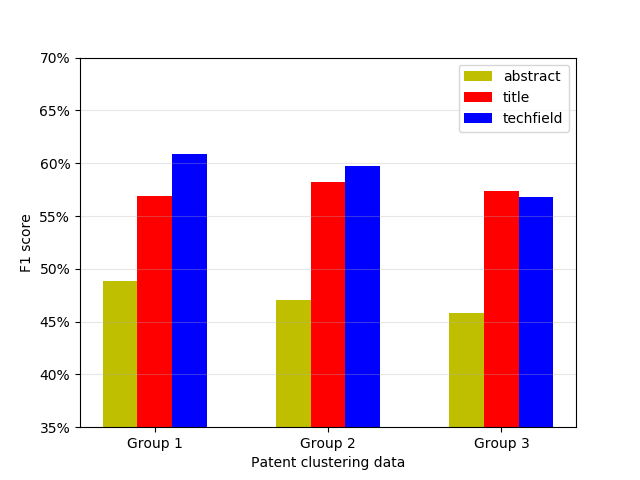
\includegraphics[scale=0.49]{zzt.png} 
		\caption{F1 scores on patent keyword extraction which use three different sections in the three groups of patents to construct patent vectors when the number of extracted keywords is 13.}
		\label{zzt}
	\end{figure}
	
	In order to consider the impact of constructing patent vectors using different sections in patents on the results of patent keyword extraction, we use abstracts, titles and technical fields of patents to construct patent vectors respectively for clustering. When the number of extracted keywords is 13, the F1 scores on patent keyword extraction which use three different sections in patents to construct patent vectors are shown in Fig.~\ref{zzt}. In Group 1 and Group 2 patent clustering data, the F1 scores on patent keyword extraction using technical field to construct patent vectors are obviously higher than using abstract and title. Therefore, it is effective on constructing patent vectors using technical field. In Group 3 patent clustering data, as described above, the clustering performance is not good, so the result on patent keyword extraction which use technical field to construct patent vectors is not good as Group 1 and Group 2.
	
	In a word, it is indeed useful for patent keyword extraction to cluster patents which use similar technical methods and enrich the semantic information between words.
	
	\section{Conclusion and Future Work}
	The patent document potentially contains many innovative technical methods. Patent keywords can help us discover the technology used in patents more efficiently.
	
	In this paper, we propose an unsupervised patent keyword extraction method based on Chinese patent clustering. We use the arithmetic mean of the word vectors of each patent technical field as the patent vector to represent each patent. Then we use BIRCH clustering model to cluster several patent vectors. The centroid of each patent cluster can be calculated easily. Next, the cosine similarity between each word vector in patent abstract and cluster centroid is computed to indicate the importance of this word. Finally, the extracted keywords for each patent document are the top n words whose word vectors have the largest similarity values with relevant cluster centroid.
	
	However, the clustering results on the patents which use similar technical methods in some technical fields are not so good. Our future work is to cluster patents on a certain category of patents, each cluster contains the patents which use the same specific technology. Moreover, we plan to add position information of each word for patent keyword extraction.
	
	%\section*{Acknowledgment}
	\end{CJK}

\bibliographystyle{IEEEtran}
\bibliography{mybibfile}

\end{document}
